\subsection{Dispatcher}
\subsubsection{Overview}Routing requests is one of the most important aspects in each web service. 
Two main reasons for that are providing user-friendly URLs and having the control on access to the service content. 
{\it E\_dispatcher} has both of them.

In order to provide mapping URL - view/controller we must fill dispatcher configuration file ({\it dispatch.conf}) properly. 
This file (placed in {\it config} directory) is read during the start of the application, 
so after making any change inside {\it dispatch.conf} (or configuration files included in it) we must force dispatcher to reload its routing table. 
It could be done by typing
\begin{verbatim}
e_dispatcher:reinstall().
\end{verbatim}

\subsubsection{Types of dispatching}There are two basic types of dispatching: {\bf static} and {\bf dynamic}.
\paragraph{Static dispatching}
Static dispatching has been designed for accessing the content which doesn't need to be generated for request (which is {\it static}). 
We can serve files directly as they are (for example some media: images, css or so): 
without inspecting the content and changing the access path, or we can point the template which should be expanded. 

In both cases we don't hit controller at all: we must know exactly what is the response for the request in the moment of creation of the dispatcher entry.
\paragraph{Dynamic dispatching}
Dynamic dispatching involves controller in handling requests. 
The URL user entered in his browser is mapped onto the call of the controller function: 
so we can build the content on the fly (fetch data from database, control the access, validate input data).

\subsubsection{Control flow}After receiving request from client, application must handle it in some way. 
At first dispatcher checks if the URL matches any of the static entries. 
If so, the dispatcher tries to get target file from {\it templates} directory. 
If it fails, it looks for it in {\it docroot} folder. In other case - when route it dynamic - dispatcher passes the request to the target controller.

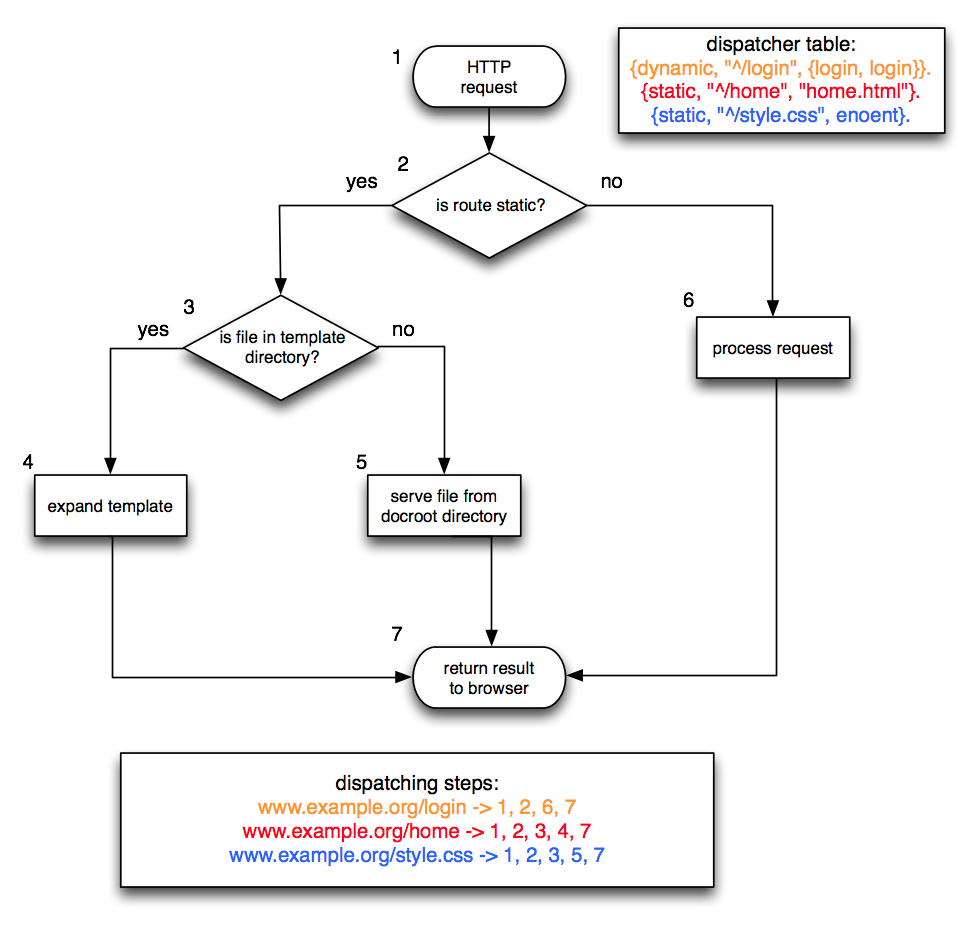
\includegraphics[width=\textwidth]{images/dispatch.jpg}

\subsubsection{dispatch.conf}{\it dispatch.conf} file is placed under {\it config} directory - is the one of the must-have files in our application. 
It consits of Erlang tuples which tell dispatcher how to handle incoming request. 

Each entry contains {\bf Regexp} element - dispatcher checks if it matches the request URL. 
First matching entry will be used to handle the request.

The following types of entries are allowed in {\it dispatch.conf} file:
\begin{itemize}
\item {\bf \{static, Regexp, File\}}

Statically dispatches the request to {\bf File}. {\bf File} should be placed in {\it templates} directory. 
If there is no file with given name, server tries to find it in {\it docroot} folder. 

To make file serving faster, we can set {\bf File} to {\bf enoent} atom - it means that server should not look for it in {\it templates} directory.
\item {\bf \{dynamic, Regexp, \{Module, Function\}\}}

{\bf Module}:{\bf Function} will be called in order to satisfy the request.
\item {\bf \{dynamic, delegate, Regexp, File\}}
To make {\it dispatch.conf} file clearer, easier to read and mantain we can use {\bf delegate} entry. 
At first dispatcher reads the {\bf File} and suffixes with {\bf Regexp} all {\bf Regexps} in entries in read file. 

This kind of entry does not have any practical meaning - it only helps to structuralize the application. 
The same effect can be achived by explicitly placing all the entries from {\bf File} in original one (with suffixed {\bf Regexp} element).
\end{itemize}

\subsubsection{Named subpatterns}Named subpatterns is the mechanism used for extracting the certain information from the input string. 
Having regular expression we are able to specify the semantic of the incoming URL and get its value.
Moreover, the named subpatterns allows us to do a simple syntax validation.

The syntax is the same as in dynamic dispatcher rules, but the regular expression is a little bit modified. 
If we want to bind some part of the input string to the given name, we should use the following syntax:
\begin{verbatim}
"HeadOfRegexp(?<NameOfThePattern>RegexpPart)TailOfRegexp"
\end{verbatim}
So when the whole regular expression matches the request URL, it will extract its selected part and tag it with the specified name. 
The list of extracted values will be passed to the first function on dataflow list (if we are not using the named subpatterns mechanisms we will get the empty list there).
The passed list will have format:
\begin{verbatim}
[{name_of_the_pattern, Value} | ...]
\end{verbatim}

For example, when we run a blog and we want to display our post by entering the address {\it /show/post/Post\_no}, we can do it using named subpatterns:
\begin{verbatim}
{dynamic, "^/blog/post/(?<post_no>[0-9]+)$", {blog, display_post}}.
\end{verbatim}
So when the incoming URL, let's say {\it "/blog/post/23"}, could be described by the regular expression: {\it "\^/blog/post/[0-9]+\$"}, 
then the part responsible for post number will be extracted from it. 
The result of the named subpatterns will be a property list: 
\begin{verbatim}
[{post_no, "23"}] 
\end{verbatim}
and it will be passed to the first function on the dataflow list.

We can place more than one named subpatterns in the regular expressions, for example:
\begin{verbatim}
{dynamic, "^/blog/post/(?<post_no>[0-9]+)/comment/(?<comment_title>.+)$}.
\end{verbatim}
for {\it "/blog/post/5/comment/first\_comment"} URL, dispatcher will pass 
\begin{verbatim}
[{post_no, "5"}, {comment_title, "first_comment"}] 
\end{verbatim}
to the first function on the dataflow list.

\subsubsection{Skipping dispatcher}
Because sometimes our service provides very simple API, we do not need dispatcher support. 
Moreover, {\it regexp} module is not as fast as Perl equivalent, 
so for efficency reasons we will decide that we want uglier URL's instead of many regular expression matches. 
The last reason for providing the dispatcher omission functionality is to keep the backward compatibility with the prior version of {\it ErlangWeb}.

If we want to skip dispatcher, we must prefix the URL with {\it app/}. 
The meaning is as follows:
\begin{Verbatim}
http://example.org/app/Module/Function/View.part1/View.part2/.../View.partN
\end{Verbatim}
The call path is split with {\bf /} and the {\it Module:Function} is called (of course following the dataflow rules). 
In case {\it Module:Function} call returns the {\it template} atom, 
the {\it View} will be expanded (path to the template will be created by joining the {\it View.partN}).

\subsubsection{Example}
This is a simple example of nested dispatcher configuration files:

\begin{Verbatim}[numbers=left, frame=single, label=dispatch.conf]
{dynamic, "^[/]*$", {main, home}}.
{dynamic, "^/index.html$", {main, home}}.

{dynamic, delegate, "^/user", "config/dispatcher/user.conf"}.

{static, "^/about$", "about.html"}.
{static, "^style.css$", enoent}.
\end{Verbatim}
and the included file:
\begin{Verbatim}[numbers=left, frame=single, label=user.conf]
{dynamic, "/create$", {users, create}}.
{dynamic, "/delete$", {users, delete}}.

{static, "/welcome$", "users/welcome.html"}.
\end{Verbatim}

The following services will be accessible on corresponding URLs:
\begin{itemize}
\item "/" $\Rightarrow$ function call {\bf main:home}
\item "index.html" $\Rightarrow$ function call {\bf main:home}
\item "style.css" $\Rightarrow$ direct access to {\it style.css} file in {\it docroot} directory
\item "about" $\Rightarrow$ expanding template {\it about.html}
\item "user/create" $\Rightarrow$ function call {\bf users:create}
\item "user/delete" $\Rightarrow$ function call {\bf users:delete}
\item "user/welcome" $\Rightarrow$ expanding template {\it users/welcome.html}
\end{itemize}
